% =====================================================================
% StaticKD -- IEEE Access manuscript (ieeeaccess class)
% Restructured on 2026-11-01 from commit b4bf5e6 by paper_writing/restructure/assemble_restructure.py.
% Numbers are literal; results/final/paper_number_map.json lists every number.
% Fig. 1 is compiled separately: cd figures && pdflatex fig_pipeline (TikZ clashes with ieeeaccess.cls).
% Compile: pdflatex main && bibtex main && pdflatex main && pdflatex main
% =====================================================================
\documentclass{ieeeaccess}
\usepackage[nocompress]{cite}
\usepackage{amsmath,amssymb,amsfonts}
\usepackage{graphicx}
\usepackage{textcomp}
\usepackage{booktabs}
\usepackage{multirow}
\usepackage{array}
\usepackage[hyphens]{url}
\usepackage{algorithm}
\usepackage{algpseudocode}

\DeclareRobustCommand{\todo}[1]{{\color{red}[TODO: #1]}}

\emergencystretch=1.5em

\begin{document}
\history{Date of publication xxxx 00, 0000, date of current version xxxx 00, 0000.}
\doi{10.1109/ACCESS.2024.0429000}

\title{StaticKD: Distilling a Multilingual IPTC News Topic Classifier into a Static Token-Logit Table for Lightweight CPU Inference}

\author{\uppercase{Obi Kastanya}\authorrefmark{1} AND \uppercase{Ananta Dwi Prayoga Alwy}\authorrefmark{1}}
\address[1]{Department of Informatics Engineering, Sepuluh Nopember Institute of Technology, Surabaya, Indonesia (e-mail: 6025252015@student.its.ac.id; 6025252007@student.its.ac.id)}
\tfootnote{This work received no specific funding.}

\markboth
{Kastanya and Alwy: StaticKD, Multilingual IPTC News Topic Classification on CPU}
{Kastanya and Alwy: StaticKD, Multilingual IPTC News Topic Classification on CPU}

\corresp{Corresponding author: Obi Kastanya (e-mail: 6025252015@student.its.ac.id).}

\begin{abstract}
Filtering news by the International Press Telecommunications Council (IPTC) Media Topic taxonomy requires a classifier cheap enough for a multilingual article stream. The open multilingual IPTC classifier based on XLM-RoBERTa-large needs 1,190 to 2,816 milliseconds per article on one processor core. StaticKD uses this classifier as teacher and gives every vocabulary token one score for each of the 17 top-level IPTC topics. Classification only requires tokenizing an article and averaging its token scores. The student is initialized from multilingual static embeddings (one fixed vector per token) and learns from teacher outputs on 285,999 articles in 69 languages. The evaluation uses a new test set of 12,744 articles in 47 languages. Its labels come from human annotators or newsroom editors and not from a model that reads the article. StaticKD reaches a macro-F1 of 0.545 on this set and keeps 91.1\% of the teacher score (0.598). The 34-megabyte model classifies 539 articles per second per core and runs about 682 times faster than the 8-bit quantized teacher. It is more accurate than fastText and a linear support vector machine trained on the same labels. A Model2Vec classifier trained on these labels is equally accurate within 0.01 macro-F1 but needs a file 15 times larger. Five-seed ablations show that accuracy comes mainly from multilingual training data and pre-trained cross-lingual embeddings. The same ablations show that the top teacher label works as well as the full distribution. StaticKD is weakest on languages absent from both its training data and the teacher's pre-training data.
\end{abstract}

\begin{keywords}
Efficient inference, knowledge distillation, multilingual text classification, news topic classification, static embeddings.
\end{keywords}

\titlepgskip=-21pt

\maketitle

\section{Introduction}
\label{sec:introduction}
\PARstart{T}{ransformer}-based models such as BERT, RoBERTa, and multilingual extensions of these models have become the dominant approach to news article classification because such models capture deep semantic representations and contextual dependencies~\cite{razuvayevskaya2024peft,sebok2025babelmachine,kuzman2025llm}. The real-world use of a news classification system requires a standardized and consistent underlying taxonomy. Many prior studies have relied on localized, fragmented, or corpus-specific label sets~\cite{razuvayevskaya2024peft,adelani2023masakhanews,mirashi2023indicnews}. The International Press Telecommunications Council (IPTC) maintains the Media Topic taxonomy as a shared standard for semantic interoperability and uniform information exchange across global media organizations~\cite{iptc2024mediatopics}. The taxonomy is a language-agnostic hierarchy with 17 top-level categories that span domains such as politics, economy, sport, and disasters.

Transformer models that map news articles onto the IPTC taxonomy are accurate but encounter computational bottlenecks in production on commodity central processing unit (CPU) servers without a dedicated graphics processing unit (GPU)~\cite{zschache2026energy,treviso2023efficient}. Multi-head self-attention has a computational and memory complexity of $O(N^2)$ with respect to the input length $N$~\cite{minaee2022dltextclf}. A transformer classifier with hundreds of millions of parameters occupies gigabytes of memory. Every layer runs dense matrix multiplications on the few CPU cores that the classifier shares with the other stages of a news pipeline.

Several research efforts have attempted to lower the cost of transformer models. Parameter-efficient fine-tuning (PEFT) methods such as Low-Rank Adaptation (LoRA) reduce memory overhead during training but provide no inference speedup because the merged model retains the full original architecture and computational cost~\cite{xu2026peftreview}. Other studies distill large transformers into compact architectures such as MiniLM~\cite{wang2021minilmv2} and DistilBERT~\cite{sanh2019distilbert}. The multilingual versions of these compact transformers hold more than 100 million parameters and keep self-attention and dense matrix multiplications. Bag-of-words models such as fastText~\cite{joulin2017bag} reach millisecond latency on CPU but transfer poorly across languages because the token vectors are learned from scratch without cross-lingual alignment.

News topic classification suits static representations because bag-of-words models remain competitive with sequence models on topic classification~\cite{galke2022bow}. Sparse Distillation~\cite{ye2022sparse} showed that the knowledge of a transformer can be transferred into a bag-of-embeddings student by minimizing the Kullback--Leibler (KL) divergence to the soft predictions of the teacher. Recent work by Wada et al.~\cite{wada2025static} and the Model2Vec framework~\cite{tulkens2024model2vec} has shown that sentence transformers can be compressed into static token embeddings. The multilingual Model2Vec embeddings are aligned across 101 languages. Singh et al.~\cite{singh2023auglinear} showed that linear classification models can be converted into coefficient lookup dictionaries that accelerate inference on CPU without a GPU. Applying a linear head to every token embedding before deployment is called folding in this paper.

The prior work leaves three gaps.
\begin{enumerate}
  \item \emph{Computational and scale gap.} The open multilingual IPTC classifier of Kuzman and Ljube\v{s}i\'c~\cite{kuzman2025llm} is an XLM-RoBERTa-large (XLM-R) model~\cite{conneau2020xlmr} with 24 transformer layers and 559.9~million parameters. Sparse Distillation~\cite{ye2022sparse} was evaluated only on English and stores about one billion parameters in its n-gram table. The coefficient dictionary of Singh et al.~\cite{singh2023auglinear} covers only the n-grams seen in training. Coefficients of new n-grams can optionally be inferred from large language model (LLM) embeddings of these n-grams.
  \item \emph{Architectural non-linearity gap.} Sparse Distillation~\cite{ye2022sparse} and the default classifier of Model2Vec~\cite{tulkens2024model2vec} place a non-linear multilayer perceptron (MLP) head on top of the averaged embeddings. The non-linear layers prevent folding the head into the embeddings and keep two matrix multiplications in every inference pass.
  \item \emph{Evaluation gap.} The human-annotated IPTC test set of Kuzman and Ljube\v{s}i\'c is not public and covers four languages. SIB-200~\cite{adelani2024sib200} covers 205 languages but consists of short sentences labeled with a non-IPTC taxonomy. No public test set offers human or editorial IPTC labels in many languages.
\end{enumerate}

The present study addresses these gaps with StaticKD and a multilingual test set. StaticKD uses the open IPTC classifier as teacher and trains a linear head over multilingual static embeddings on teacher-labeled news in many languages. The head is then folded into the embeddings so that classification reduces to averaging the rows of one token table. The test set draws on news pages whose publishers record the newsroom section in the page metadata (schema.org~\cite{guha2016schema}). It also includes public datasets that carry human annotations or publisher categories~\cite{adelani2023masakhanews,petukhova2023mnds,mirashi2023indicnews,hossain2025banglanews}. Every label was mapped onto the IPTC taxonomy without a model that read the article text.

The study answers four research questions (RQs). RQ1 asks how much of the teacher accuracy StaticKD retains on labels that do not come from the teacher. It also compares StaticKD with other light classifiers and with small transformers. RQ2 concerns the inference cost of the teacher on CPU and how far StaticKD reduces that cost. RQ3 examines which parts of the training recipe matter for this small student. RQ4 looks for the languages, labels, and label sources on which StaticKD is weak.

The main contributions of this study are as follows.
\begin{itemize}
  \item A lightweight multilingual IPTC classifier that runs on CPU as a single token-logit table without a deep learning library.
  \item A multilingual IPTC test set with editorial labels that is released as a manifest with a reconstruction script and the section-to-IPTC mapping table.
\end{itemize}

Section~\ref{sec:related} reviews related work. Section~\ref{sec:method} describes StaticKD. Section~\ref{sec:data} describes the data and the test set. The baselines and the evaluation protocol are given in Section~\ref{sec:setup}. The results are presented in Section~\ref{sec:results} and discussed together with the limitations of the study in Section~\ref{sec:discussion}. Section~\ref{sec:conclusion} concludes the paper.

\section{Related Work}
\label{sec:related}
\subsection{Multilingual News Classification and the IPTC Taxonomy}
\label{sec:rw-iptc}
The IPTC Media Topic taxonomy~\cite{iptc2024mediatopics} offers one shared scheme in place of the ad-hoc labeling schemes of individual newsrooms. The top level of the taxonomy has 17 categories such as politics, economy, sport, crime, and disasters.

Datasets for news topic classification usually define a dataset-specific taxonomy and cover only one language or one region. Human annotators labeled the news articles of MasakhaNEWS~\cite{adelani2023masakhanews} with seven categories. The dataset covers English, French, and 14 other languages widely spoken in Africa. L3Cube-IndicNews for 10 Indian languages~\cite{mirashi2023indicnews} and a Bangla news dataset~\cite{hossain2025banglanews} take labels from publisher site categories. MN-DS~\cite{petukhova2023mnds} is the only public dataset annotated by humans directly with top-level IPTC topics. Its articles are in English only.

Expert annotation of news in dozens of languages is expensive. Recent work uses zero-shot LLMs as annotators to avoid this cost. Fatemi et al.~\cite{fatemi2023gptiptc} evaluated GPT for zero-shot classification of news articles into the IPTC taxonomy. Kuzman and Ljube\v{s}i\'c~\cite{kuzman2025llm} built the EMMediaTopic corpus~\cite{emmediatopic2025} by using GPT-4o to annotate news articles in four European languages (Slovenian, Croatian, Catalan, and Greek). The silver-standard data were used to fine-tune the XLM-R-large contextual transformer~\cite{conneau2020xlmr} with 559.9~million parameters. The resulting model performs on par with GPT-4o on a human-annotated test set. A later study by the same group found that fine-tuned encoders are more practical than LLMs for large-scale annotation~\cite{kuzman2025southslavic}. Studies in computational social science report that LLM annotations of political text and sentiment can reach agreement comparable to that of human coders~\cite{heseltine2024llmannotation,bojic2025llmvshuman}.

The fine-tuned model is the teacher of the present study (Section~\ref{sec:teacher}). The teacher stacks 24 transformer layers with multi-head self-attention and was fine-tuned on only four languages. Its accuracy in other languages rests on cross-lingual transfer from XLM-R pre-training. No inexpensive IPTC classifier has yet been evaluated on real news in many languages.

\subsection{Knowledge Distillation into Bag-of-Embeddings Architectures}
\label{sec:rw-kd}
Knowledge distillation (KD) transfers the knowledge encoded in a cumbersome teacher network into a lightweight student model by aligning the output probability distributions of both models~\cite{hinton2015distilling,gou2021kdsurvey,gupta2022compression}. The logit vectors of the teacher and the student are both divided by a temperature $\tau$ before the softmax. A higher $\tau$ flattens the distribution and thus shows the student how much probability the teacher assigns to the wrong classes. The full distribution is called a soft label. The top class alone is called a hard label. Students for text classification are almost always transformers such as DistilBERT~\cite{sanh2019distilbert} or MiniLMv2~\cite{wang2021minilmv2}. The same holds for cross-lingual distillation that transfers teacher knowledge to languages with little data~\cite{piperno2025crosslingual}.

Ye et al.~\cite{ye2022sparse} introduced Sparse Distillation and showed that large transformers such as RoBERTa-large can be distilled into non-contextual bag-of-embeddings representations by minimizing the KL divergence to the soft predictions of the teacher. The student retains 97\% of the accuracy of the teacher on six English classification tasks and runs up to 600 times faster. The word and n-gram embedding table of the student holds about one billion parameters and needs gigabytes of storage. The pooled representation $\mathbf{h}(d)$ of this deep averaging network~\cite{iyyer2015dan} passes through two fully connected layers with a rectified linear unit (ReLU) in between:
\begin{equation}
\mathbf{z}^S(d)=W_2\cdot\max(0,W_1\mathbf{h}(d)+\mathbf{b}_1)+\mathbf{b}_2.
\label{eq:mlp}
\end{equation}
The non-linear operator $\max(0,\cdot)$ prevents folding the head into the embedding table. The student keeps two dense matrix multiplications at inference and cannot be reduced to an additive lookup table. Sparse Distillation was also validated only on English benchmarks.

The success of distillation depends on the capacity gap between teacher and student. The optimal teacher size for language models even follows an empirical law with respect to the student size~\cite{zhang2025law}. Temperature is treated as an important hyperparameter that can be learned~\cite{li2023ctkd}. The KL divergence can be split into a target-class part and a non-target part (dark knowledge)~\cite{zhao2022dkd}. A recent analysis~\cite{wang2026rckd} shows that KL distorts the ranking of classes when the capacities of the teacher and the student do not match. High agreement between student and teacher does not always come with better generalization~\cite{stanton2021kd}. Nearly all of these findings come from deep students. StaticKD faces a gap from 559.9~million parameters to one linear layer over averaged embeddings. No study has yet characterized how temperature and soft labels behave at such an extreme gap.

\subsection{Multilingual Static Embedding Compression (Model2Vec)}
\label{sec:rw-static}
Classical static embeddings such as fastText~\cite{joulin2017bag} provide rapid CPU execution by representing a document as the average of its token vectors. The fastText vectors are learned from scratch without cross-lingual alignment and transfer poorly to other languages.

The Model2Vec framework~\cite{tulkens2024model2vec} introduced a post-processing distillation technique that compresses sentence transformers into static token embeddings. Wada et al.~\cite{wada2025static} propose a related method that refines static embeddings extracted from a sentence transformer. The multilingual model potion-multilingual-128M is distilled from BGE-M3~\cite{chen2024bgem3} and holds an aligned embedding matrix $E\in\mathbb{R}^{|V|\times d_e}$ with $d_e=256$ and $|V|=500{,}353$ for 101 languages. Translation equivalents lie close to each other in this space because the alignment is inherited from the multilingual sentence encoder.

The classifier of the Model2Vec library (\texttt{StaticModelForClassification}) adds a non-linear hidden layer of 512 units by default~\cite{tulkens2024model2vec}. Its head has the same form as \eqref{eq:mlp} and is trained with cross-entropy on hard labels. The hidden layer keeps two matrix multiplications in every inference pass and prevents folding in the same way as the head of Sparse Distillation.

Static embeddings are usually evaluated as general-purpose embeddings rather than as distillation students for a specific taxonomy.

\subsection{Analytic Folding of Linear Text Classifiers}
\label{sec:rw-fold}
Singh et al.~\cite{singh2023auglinear} showed in the Aug-Linear framework that a linear model over embeddings of n-grams can be converted into a dictionary of additive coefficients. Inference needs one lookup per n-gram and a single sum. A linear head commutes with the averaging of token embeddings and can be applied to every embedding once before deployment. Inference reduces to gathering and averaging rows of a precomputed table (Section~\ref{sec:fold}). Singh et al. applied the folding to n-gram vocabularies with hard labels in a binary classification setting. Coefficients for n-grams unseen in training can optionally be inferred from LLM embeddings of these n-grams. The formulation uses no distillation from a teacher and was evaluated on English datasets.

\subsection{Test Sets with Editorial Labels, Contamination, and Sample Dependence}
Earlier work has used publisher site categories as topic labels mostly for one publisher or one region~\cite{mirashi2023indicnews}. Many news sites also record the section of each article in the \texttt{articleSection} field of the machine-readable schema.org page metadata~\cite{guha2016schema}. The field has not yet been mapped to a standard taxonomy across dozens of languages. Leakage between training and test data also has to be controlled. Near-duplicate removal with MinHash~\cite{broder1997resemblance} has become standard practice~\cite{lee2022dedup}. Significance tests in natural language processing such as the paired bootstrap~\cite{koehn2004significance} usually assume independent samples~\cite{dror2018hitchhiker}. Articles from the same site depend on each other. The cluster bootstrap~\cite{field2007bootstrapping} handles this dependence by resampling clusters instead of documents.

\subsection{The StaticKD Architectural Synthesis}
StaticKD combines elements of four lines of work.
\begin{itemize}
  \item The teacher and its distribution over the 17 IPTC topics come from Kuzman and Ljube\v{s}i\'c (Section~\ref{sec:rw-iptc}).
  \item KL distillation into a bag-of-embeddings student follows Sparse Distillation (Section~\ref{sec:rw-kd}) without its billion-parameter n-gram table and non-linear head.
  \item The aligned potion-multilingual embedding space ($d_e=256$) comes from Model2Vec (Section~\ref{sec:rw-static}) without its non-linear classifier.
  \item The folding identity comes from Singh et al. (Section~\ref{sec:rw-fold}) and is applied to a closed multilingual subword vocabulary ($|V|=500{,}353$).
\end{itemize}
The strictly linear head allows exact folding of the trained weights into one half-precision table. Inference runs in NumPy and needs no dense matrix multiplication, no GPU, and no deep learning library. The position of StaticKD relative to these related approaches is summarized in Table~\ref{tab:related}.

\begin{table*}[!t]
\caption{Position of StaticKD Relative to Related Approaches}
\label{tab:related}
\centering
\footnotesize
\setlength{\tabcolsep}{4pt}
\resizebox{\textwidth}{!}{%
\begin{tabular}{@{}llccccc@{}}
\toprule
Approach & Model at inference time & Multilingual & Cross-lingual transfer & No deep learning library & CPU cost reported & IPTC labels \\
\midrule
Kuzman \& Ljube\v{s}i\'c~\cite{kuzman2025llm} & XLM-R-large (559.9M parameters) & yes & yes & no & no & yes \\
DistilBERT, MiniLMv2~\cite{sanh2019distilbert,wang2021minilmv2} & 6-layer transformer & partly & yes & no & partly & no \\
Sparse Distillation~\cite{ye2022sparse} & deep averaging network + n-gram table & no (en) & no & yes & yes & no \\
Model2Vec~\cite{tulkens2024model2vec}, Wada et al.~\cite{wada2025static} & static embeddings, optional MLP classifier & yes & yes & yes & partly & no \\
fastText~\cite{joulin2017bag} & bag of n-grams & per language & no & yes & yes & no \\
StaticKD (proposed) & table of 17 logits per token & yes & yes & yes & yes & yes \\
\bottomrule
\end{tabular}}
\end{table*}

\section{The StaticKD Method}
\label{sec:method}
\subsection{Study Overview}
\label{sec:overview}
The study consists of three main stages: building the StaticKD student by distillation, measuring and comparing accuracy on labeled articles that neither the teacher nor the student has seen, and measuring the inference cost on CPU.

Fig.~\ref{fig:pipeline} shows the StaticKD pipeline that this study builds. The teacher classifies 285,999 unlabeled articles in 69 languages and produces logits for the 17 top-level IPTC topics (Sections~\ref{sec:distdata} and~\ref{sec:teacher}). Logits are the raw scores that a model outputs for each class before the scores are converted into probabilities. The StaticKD model is trained to imitate the teacher distribution over the 17 IPTC topics (Section~\ref{sec:student}).

Teacher labels do not serve as ground truth in this study. Prediction accuracy is evaluated on a separate test set with editorial labels (Section~\ref{sec:testset}). The CPU benchmark of the third stage runs every model on the same sample of test articles (Section~\ref{sec:effprotocol}).

\begin{figure*}[!t]
\centering
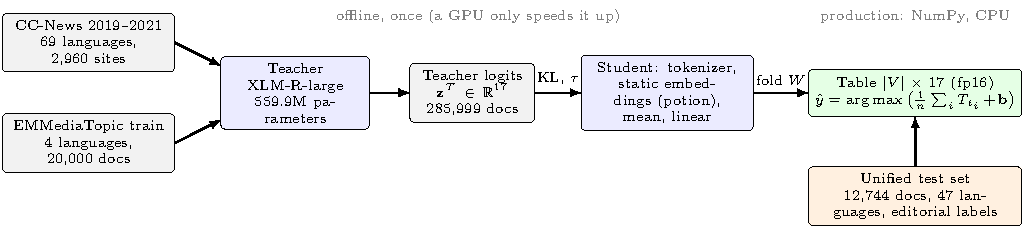
\includegraphics[width=\textwidth]{figures/fig_pipeline.pdf}
\caption{StaticKD pipeline. The teacher labels an unlabeled news corpus once in an offline step. The student learns to imitate the teacher distribution. Its linear head is then folded into a token table. Inference reduces to a lookup and an average of table rows. The final evaluation uses a test set whose labels do not come from the teacher.}
\label{fig:pipeline}
\end{figure*}

\subsection{Problem Formulation}
A model predicts one label $y\in\mathcal{Y}$ among the 17 top-level IPTC topics for a news article $d$ in any language. The input is the title and body truncated to the first 512 words as in~\cite{kuzman2025llm}. The teacher $f_T$ outputs logits $\mathbf{z}^T(d)\in\mathbb{R}^{17}$. The goal is a student $f_S$ whose inference costs $O(n)$ additions for $n$ tokens and needs neither matrix multiplication nor a deep learning library. Its accuracy against independent labels should be as close as possible to that of $f_T$.

\subsection{Teacher and Distillation Labels}
\label{sec:teacher}
The teacher is the IPTC classifier of~\cite{kuzman2025llm} published as \url{classla/multilingual-IPTC-news-topic-classifier}. It is an XLM-RoBERTa-large model with 24 layers, 559.9 million parameters, and an input limit of 512 XLM-R tokens. The 512-word input exceeds this limit for 60.7\% of the test articles. The teacher reads about 287 of the 438 words of such an article (medians). The full logit vector $\mathbf{z}^{T}(d)\in\mathbb{R}^{17}$ of the teacher was stored for every distillation document. Labeling all distillation data was a one-time cost of about 1.6 GPU hours.

\subsection{The StaticKD Student}
\label{sec:student}
The student in this study is built on the multilingual static embedding model potion-multilingual-128M of Model2Vec~\cite{tulkens2024model2vec} (hereafter potion). A document $d$ is tokenized into $t_1,\dots,t_n$ with the Unigram tokenizer of potion so that every token has a pre-trained embedding. The tokenizer contains 500,353 tokens. Special tokens are not used and unknown tokens are dropped. The document length is capped at 1,024 tokens. The cap only serves to bound the cost because averaging does not depend on position. Only 5.4\% of the test articles exceed it. Each token has an embedding $\mathbf{e}_t\in\mathbb{R}^{256}$ and
\begin{equation}
\mathbf{h}(d)=\frac{1}{n}\sum_{i=1}^{n}\mathbf{e}_{t_i},\qquad
\mathbf{z}^{S}(d)=W\,\mathrm{drop}(\mathbf{h}(d))+\mathbf{b},
\label{eq:student}
\end{equation}
with $W\in\mathbb{R}^{17\times 256}$ and dropout 0.1 during training. The embedding matrix $E$ is initialized from potion. The potion model itself was distilled from BGE-M3~\cite{chen2024bgem3} and covers 101 languages. The potion initialization places the tokens of these 101 languages in one shared space before training starts.

The student learns from the stored teacher logits with the loss
\begin{equation}
\mathcal{L}_{\mathrm{KD}}=\tau^{2}\,\mathrm{KL}\!\left(p^{T}\,\middle\|\,p^{S}\right),\qquad \tau=1 ,
\label{eq:kd}
\end{equation}
where $p^{T}=\mathrm{softmax}(\mathbf{z}^{T}/\tau)$ and $p^{S}=\mathrm{softmax}(\mathbf{z}^{S}/\tau)$ are the teacher and student distributions. The value $\tau=1$ was chosen during development. The results for $\tau\in\{0.5,2,4\}$ are reported in Section~\ref{sec:res-abl}. The parameters $E$, $W$, and $\mathbf{b}$ are trained together. SparseAdam ($\eta=10^{-3}$) updates the embedding matrix $E$ only in the rows of tokens that occur in the current batch. Tokens that never occur in the training documents therefore keep the potion embeddings. AdamW ($\eta=3\cdot 10^{-3}$, weight decay $10^{-4}$) is used for $W$ and $\mathbf{b}$. Training runs for 6 epochs with a batch size of 64. Training also applies token dropout as a cheap augmentation. Each token of a training document is dropped with probability 0.2 at every step so that the model does not rely on a few keywords. Internal validation uses 3\% of the distillation data (8,579 documents) to keep the epoch with the highest agreement with the teacher.

\subsection{Folding, Table Ensemble, and Compact Variant}
\label{sec:fold}
The linear classification head allows \eqref{eq:student} to be rewritten as
\begin{equation}
W\Big(\frac{1}{n}\sum_{i}\mathbf{e}_{t_i}\Big)+\mathbf{b}=\frac{1}{n}\sum_{i}T_{t_i}+\mathbf{b},
\label{eq:fold}
\end{equation}
with the table $T=EW^{\top}\in\mathbb{R}^{|V|\times 17}$. The folding step computes $T$ once after training. Row $T_t$ holds the 17 topic scores that token $t$ contributes to every article that contains it. The deployed model consists only of $T$ (fp16), $\mathbf{b}$, and the tokenizer. Algorithm~S1 in the supplementary material lists the whole inference procedure. The same argument holds for an ensemble because Equation~\eqref{eq:fold} is linear in $T$. Averaging the logits of $K$ students trained with different seeds gives the same result as one student with table $\bar{T}=\frac{1}{K}\sum_k T^{(k)}$ and bias $\bar{\mathbf{b}}$. The final StaticKD model averages the tables of three such students ($K=3$). It has 8.5 million parameters and a size of 34~MB.

The table itself takes 16~MB. Most of the random-access memory (RAM) goes to the internal structure of the Unigram tokenizer. A compact variant shrinks this structure by removing token pieces that occur fewer than 10 times in the distillation data. It keeps single characters and has a vocabulary of 335,441 tokens and a model size of 23~MB. The hyperparameters of all models are listed in Table~S1 of the supplementary material.

\section{Data and Test Set}
\label{sec:data}
\subsection{Data Sets and Their Roles}
\label{sec:roles}
Table~\ref{tab:datasets} lists the data sets used in this study. The development set is the development split of EMMediaTopic (1,000 articles in four languages with GPT-4o labels). All parameter settings and recipe choices for StaticKD were made on this set. The recipe was fixed \emph{before} the test set was built. A set of 320 LLM-labeled articles described in the supplementary material also informed two of these choices: the temperature $\tau=1$ and the three-seed ensemble.

\begin{table}[!t]
\caption{Data Sets of the Study and Their Roles}
\label{tab:datasets}
\centering
\footnotesize
\setlength{\tabcolsep}{3pt}
\resizebox{\columnwidth}{!}{%
\begin{tabular}{@{}lrrll@{}}
\toprule
Set & Docs & Lang. & Labels & Used for \\
\midrule
Distillation data & 285,999 & 69 & teacher & training the students \\
\quad internal validation & 8,579 & -- & teacher & choosing the epoch \\
Development (EMMediaTopic) & 1,000 & 4 & GPT-4o & choosing the recipe \\
CC-News held-out & 12,554 & 63 & teacher & agreement, unseen sites \\
Unified test set & 12,744 & 47 & editorial & all accuracy results \\
English section sample & 754 & 1 & JSON-LD & label validity only \\
\bottomrule
\end{tabular}}
\end{table}

\subsection{Distillation Data and Development Set}
\label{sec:distdata}
The distillation data and the development set both draw on EMMediaTopic 1.0~\cite{emmediatopic2025,kuzman2025llm}. EMMediaTopic was labeled with GPT-4o and consists of articles in four languages (Catalan, Greek, Croatian, and Slovenian). A total of 21,000 annotated articles were taken and divided into a training split of 20,000 and a development split of 1,000 articles. Kuzman and Ljube\v{s}i\'c used the training split to train the teacher. The same split also forms part of the distillation data for the student. The development split was never used to train the teacher or the student. Kuzman and Ljube\v{s}i\'c used the development split to tune the hyperparameters of the teacher~\cite{kuzman2025llm}.

A large part of the distillation data comes from the multilingual CC-News 2019--2021 dataset~\cite{cloversearch_ccnews} built from the news archive of Common Crawl. The test set was drawn from CC-News for a different range of years (CC-NEWS 2024--2026, Section~\ref{sec:testset}). CC-News 2019--2021 was processed with the following steps.
\begin{enumerate}
  \item Verify the language with the fastText language identification model~\cite{joulin2017bag} and keep only documents whose metadata language agrees with the identified language.
  \item Keep documents whose title and body reach 75 words in total and truncate the text to 512 words. Documents in ja, zh, th, and my use limits of 200 and 2,000 characters instead.
  \item Keep at most 150 documents per site.
  \item Set aside all documents of some sites as a held-out split that holds at most 20\% of each language.
  \item Add 156,157 documents from training sites only (at most 5,000 per language and 400 per site).
\end{enumerate}
The distillation data contain 285,999 documents in 69 languages from 2,960 sites. The median document length is 269 words. The number of documents per site was capped to avoid bias from similar content within one site. The held-out set contains 12,554 documents in 63 languages from 217 sites that never occur in the distillation data. It can only measure \emph{agreement} with the teacher because it has no independent category labels. Agreement is the share of documents whose top predicted label is the same as the top label of the teacher.

\subsection{Unified Test Set Construction}
\label{sec:testset}
The largest source is the CC-NEWS 2024--2026 dataset~\cite{commoncrawl2026ccnews} sampled as one archive file (WARC) per month from January 2024 to August 2026 (32 files). The schema.org JSON-LD blocks~\cite{guha2016schema} of each article page supplied metadata fields such as \texttt{articleSection}, \texttt{BreadcrumbList}, \texttt{inLanguage}, \texttt{datePublished}, \texttt{isAccessibleForFree}, and \texttt{articleBody}. The text was taken from \texttt{articleBody} only when it had at least 30 words. The text of articles without such an \texttt{articleBody} came from the HTML content through the Trafilatura library~\cite{barbaresi2021trafilatura}. The site filter removed articles from sites that already appear in the distillation data or in an evaluation set.

The other test articles come from public datasets. MasakhaNEWS~\cite{adelani2023masakhanews} and MN-DS~\cite{petukhova2023mnds} are labeled by humans. L3Cube-IndicNews (LDC split)~\cite{mirashi2023indicnews}, Bangla news~\cite{hossain2025banglanews}, and IndoNews~\cite{indonews2021} carry publisher categories.

Section and category labels record where the newsroom placed an article when it was published. Such labels are called \emph{editorial labels} in this paper. Editorial labels do not follow the IPTC standard. The section names have to be translated onto the official IPTC Media Topic tree (1,085 active nodes). The section names were first normalized for case and diacritics and then mapped conservatively by an LLM (Claude Opus 5.5). The LLM mapped a name only if the content under that section fit a single top-level topic. The mapping links 814 section names to 79 IPTC nodes. An automatic check verified that every target node exists in the IPTC tree, is not retired, and lies under the intended top-level topic. Articles whose sections mapped to different labels were rejected. The mapping table drafted by the LLM was then reviewed manually by two researchers in a joint session.

Quality and leakage filters were applied in order.
\begin{enumerate}
  \item Publication date on or after 1 January 2024 (CC-NEWS only).
  \item Not behind a paywall.
  \item Declared language agrees with fastText language identification when fastText supports the language.
  \item At least 75 words.
  \item Deduplication of uniform resource locators (URLs), identical texts, and near-duplicates (MinHash~\cite{broder1997resemblance}, Jaccard $\ge 0.7$~\cite{lee2022dedup}) across all sources.
  \item Contamination: an article was dropped when $\ge 30\%$ of its word 8-grams occurred in any of about 300 thousand training or evaluation documents. The filter removed 63 articles. Most of the removed articles came from MasakhaNEWS. MasakhaNEWS also draws on BBC.
\end{enumerate}

Sampling took at most 50 articles for each pair of language and label. The priority order was human-labeled sources first, publisher categories second, and JSON-LD sections last. The number of articles per site was not capped. Languages with fewer than 30 articles were dropped.

The final test set contains 12,744 articles in 47 languages from 1,227 sites or sources. All 17 labels occur in it. The articles of a language cover a median of 7 of the 17 labels. The median article length is 313 words. Human annotators labeled 4,094 of these articles (32.1\%). Publisher categories cover 2,600 (20.4\%) and JSON-LD sections 6,050 (47.5\%). The label type of an article (human annotation, publisher category, or JSON-LD section) is called its \emph{label origin}. No distillation data exist for 13 languages (e.g., ha, yo, ig, bn, and pa). Another 9 languages have fewer than 500 distillation documents. The remaining 25 languages have at least 500. The effective number of sites $1/\sum_s q_s^{2}$ measures site diversity. The quantity $q_s$ is the share of the articles of a language that come from site $s$. A source dataset without URLs counts as one site. Thirteen languages have at least 10 effective sites by this measure. Another 27 languages have fewer than 3 effective sites. One site supplies at least 90\% of the articles in 22 of these languages. Table~\ref{tab:testset} summarizes the composition of the article sources. Fig.~S1 in the supplementary material shows the number of articles of each language per label.

\begin{table}[!t]
\caption{Composition of the Unified Test Set by Source}
\label{tab:testset}
\centering
\footnotesize
\setlength{\tabcolsep}{3pt}
\resizebox{\columnwidth}{!}{%
\begin{tabular}{@{}llrrr@{}}
\toprule
Source & Label origin & Articles & Languages & Sites/sources \\
\midrule
CC-NEWS 2024--2026 & JSON-LD section & 6,050 & 29 & 1,092 \\
MasakhaNEWS~\cite{adelani2023masakhanews} & human annotation & 3,339 & 16 & 6 \\
L3Cube-IndicNews~\cite{mirashi2023indicnews} & publisher category & 2,361 & 10 & 1 \\
MN-DS~\cite{petukhova2023mnds} & human annotation & 755 & 1 & 127 \\
Bangla news~\cite{hossain2025banglanews} & publisher category & 139 & 1 & 1 \\
IndoNews & publisher category & 100 & 1 & 1 \\
\midrule
Total & & 12,744 & 47 & 1,227 \\
\bottomrule
\end{tabular}}
\end{table}

\subsection{Label Validity Check}
\label{sec:validity-design}
Two thirds of the test labels are section and category labels that record newsroom decisions rather than annotation that follows a labeling guideline. The check tests whether such labels behave like human labels in the same language (Section~\ref{sec:res-validity}). It compares how well one and the same teacher agrees with each label type. The teacher serves only as a fixed reference. Much noisier section labels would make the teacher agree less with section labels than with human labels in the same language.

The English part of the test set contains only human labels because the sampling preferred human-labeled sources (Section~\ref{sec:testset}). A comparison within English therefore uses a separate sample of articles that are not in the test set. The sample contains 754 English CC-NEWS articles with JSON-LD section labels and at most 50 articles per label. The articles come from 306 sites. The test set itself allows a comparison in French between section labels and the human labels of MasakhaNEWS. A per-category analysis in languages covered by XLM-R pre-training compares the predictions of the teacher with the mapped label of each source category.

\section{Experimental Setup}
\label{sec:setup}
\subsection{Baselines}
\label{sec:baselines}
All baselines marked + KD used the same distillation data (285,999 documents) and targets from the same teacher. The standard training procedures of the three light baselines accept class labels but not probability distributions. The fastText + KD baseline~\cite{joulin2017bag} was trained on the top teacher label with word tokens and character n-grams or with XLM-R subwords. Its quantized variant (\texttt{.ftz}) was included as well. A fastText model was also trained only on the GPT-4o labels of the EMMediaTopic training split. It serves as a reference trained on the same labeled data as the teacher~\cite{kuzman2025llm}. The non-neural baseline comes from Kuzman and Ljube\v{s}i\'c and uses term frequency--inverse document frequency (TF-IDF) features with a support vector machine (SVM). Its TF-IDF + SVM + KD version was trained on the top teacher label over XLM-R subwords. A grid search on the development set chose the hyperparameters of TF-IDF + SVM + KD and of both fastText + KD models. All values are listed in Table~S1 of the supplementary material. The Model2Vec classifier + KD was trained on the top teacher label with the classifier trainer of the Model2Vec library~\cite{tulkens2024model2vec} with its default settings. It fine-tunes the same potion embeddings that StaticKD starts from. The classifier also learns a weight for each token and adds a hidden layer of 512 units. MiniLM-L6 + KD uses mMiniLMv2-L6-H384 distilled from XLM-R-large~\cite{wang2021minilmv2}. It is trained with the loss in~\eqref{eq:kd} on the full teacher distribution. The temperature $\tau\in\{1,2\}$ for this model was chosen on the development set. The same recipe with $\tau=1$ was applied to DistilmBERT + KD with \texttt{distilbert-base-multilingual-cased}~\cite{sanh2019distilbert}. Both transformers read at most 256 tokens. The 256-token limit truncates 91.1\% of the test articles to about 142 words for MiniLM-L6 and 93.2\% to about 116 words for DistilmBERT. A sensitivity check retrained both models with 512 tokens (Section~\ref{sec:res-acc}). Both were exported to the Open Neural Network Exchange (ONNX) format in fp32 for the CPU benchmark. The teacher was also exported to ONNX with dynamic quantization to 8-bit integers (int8). The ONNX int8 teacher is the fastest teacher configuration on CPU.

Sparse Distillation~\cite{ye2022sparse} is the prior method closest to StaticKD. It was not run as a separate baseline (Section~\ref{sec:limitations}). Two other experiments still cover parts of the method. The fastText + KD baseline trained a bag-of-n-grams model with averaging and a linear head on the same teacher labels. The random-initialization ablation (Section~\ref{sec:design}) trained the embedding table from scratch as Sparse Distillation does.

\subsection{Evaluation Protocol and Statistical Tests}
\label{sec:protocol}
Macro-F1 serves as the main metric because the label distribution is imbalanced. The metric covers the labels present in the reference and is computed in the same way as in the evaluation code of~\cite{kuzman2025llm}. The evaluation also reports accuracy, agreement with the teacher on the held-out set, and macro-F1 per language. The per-language macro-F1 is averaged over languages so that large languages do not dominate.

The 95\% confidence intervals were computed by a percentile bootstrap of 1,000 resamples. The resampling unit on the test set is the site. Articles without a URL are grouped by source dataset. Such a site-cluster bootstrap~\cite{field2007bootstrapping} draws whole sites so that related articles from one site do not make the intervals too narrow. The 1,227 clusters of the test set differ in size. The two largest clusters (bbc.com and L3Cube-IndicNews) hold 37.3\% of the articles. Let $q_c$ be the share of cluster $c$. The effective number of clusters $1/\sum_c q_c^{2}$ is then only 13.8. A leave-one-source-out check therefore recomputed the macro-F1 of nine models once without each of the six test-set sources. Another check repeated the model comparison on a subset with at most five articles per site and language--label pair. The development set was resampled by document. Two models tested on the same documents were compared with a paired (cluster) bootstrap of 2,000 resamples for $\Delta$macro-F1~\cite{koehn2004significance} and an exact McNemar test for accuracy~\cite{mcnemar1947}. Holm correction~\cite{holm1979} was applied within each set. Each ablation variant ran with five seeds and the final recipe with ten. The score of an ensemble of $K$ students is the mean score over all combinations of $K$ of the ten final-recipe seeds. The same paired bootstrap compared each variant with the final recipe. Every resample scored all seeds of the variant and of the final recipe on the same articles. The tested quantity is the difference between the two seed means. Holm correction covered the 10 variants of Section~\ref{sec:design} and the four additions with three seeds each in Table~S6 of the supplementary material. A difference that is not significant does not show that two models are equivalent. Claims of equivalence rest on two one-sided tests (TOST)~\cite{schuirmann1987tost} over the same bootstrap distribution. Two models count as equivalent when the 90\% interval of $\Delta$macro-F1 lies within $\pm$0.01. The margin of 0.01 macro-F1 was treated as a negligible difference for topic filtering. A Wilcoxon signed-rank test on per-language macro-F1 and accuracy~\cite{dror2018hitchhiker} checked whether a difference is consistent across languages.

Subgroup analyses split the results by language, script, and region. The label and its origin defined further splits. The remaining subgroups were defined by site diversity, the amount of distillation data of the language, and teacher pre-training coverage. Pre-training coverage refers to whether the language is among the 100 languages used to pre-train XLM-R~\cite{conneau2020xlmr}. Spearman correlations measured the relation between per-language properties and performance. A Kruskal--Wallis test compared scripts. The $p$-values of these seven tests were Holm-corrected together. Correlations on the held-out set used the 53 languages with at least 20 held-out documents. The per-language analysis used two quantities. The \emph{accuracy gap} is the StaticKD accuracy minus the teacher accuracy. A negative gap means that StaticKD is less accurate. The \emph{token coverage} of a language is computed over all token occurrences in its test articles. Its value is the share of occurrences whose token occurs at least 10 times in the distillation data. Training seldom updates the embeddings of less frequent tokens (Section~\ref{sec:student}). The \emph{specificity} of a token is the largest difference between one entry of its table row and the mean of the other 16 entries. A pruning test kept only the 10\% most specific tokens of each article and compared the result with that of a random 10\% of the tokens. Calibration was measured with the expected calibration error (ECE, 15 bins)~\cite{guo2017calibration} because the cascade mode in Section~\ref{sec:effprotocol} routes articles by the confidence of StaticKD.

\subsection{Efficiency Protocol}
\label{sec:effprotocol}
The benchmark ran only on CPU with the GPU hidden. Each model ran in a fresh process with the thread count pinned in every library. Latency (p50 and p95) was measured with one article per call as in a streaming setting. Throughput was measured with batches of 64. The transformers used batches of 8. Model RAM is the increase in resident set size after the model is loaded. All models used the same text sample drawn at random from the unified test set. The teacher and the transformers used 100 documents for latency and 96 documents for throughput. The light models used 500 documents for latency and 3,000 documents for throughput. The whole benchmark was repeated in three separate sessions on an idle machine. The tables report the median of the three sessions. A separate single-thread profile of StaticKD timed tokenization and table averaging on 1,280 articles. The teacher stops at 512 tokens. StaticKD reads up to 1,024 tokens per article. The speed comparison therefore does not favor StaticKD. The cascade mode lets StaticKD decide the articles on which its top probability is at least a threshold $\theta$. The remaining articles are passed to the ONNX int8 teacher. Let $s$ be the share of articles decided by StaticKD and let $r_S$ and $r_T$ be the single-core throughputs of StaticKD and the teacher. The effective throughput of the cascade is then $1/(1/r_S+(1-s)/r_T)$.

The machine is a laptop with an Intel Core Ultra~7 155H, 32~GB of RAM, and Windows~11. Its CPU is hybrid and has 6 performance cores (P-cores), 8 slower efficiency cores (E-cores), and 2 low-power E-cores. The operating system moves unpinned threads to the slow cores. Each process was therefore pinned to one or four physical P-cores. The pinned setup approximates a small server with uniform cores.

\subsection{Ablation Design}
\label{sec:design}
Table~\ref{tab:ablation} lists all 60 runs of the final recipe and its ablations. Each ablation variant changes one factor of the final recipe. One variant replaces the soft labels with hard labels. Two variants reduce the training data either to EMMediaTopic only (4 languages, 10 epochs) or to 130 thousand documents without the extra CC-News 2019--2021 data. Other variants freeze the embeddings or draw random embeddings with the same standard deviation as potion. The remaining variants train without token dropout, use a 512-unit MLP head, or set $\tau\in\{0.5,\,2,\,4\}$. Four additions to the recipe tested during development are reported in Table~S6 of the supplementary material.

\subsection{Implementation Details}
\label{sec:impl}
An average StaticKD run took 5.2 minutes on an NVIDIA RTX~4050 Laptop GPU. The implementation uses Python~3.12, NumPy~2.5, PyTorch~2.6, transformers~5.17, \texttt{tokenizers}~0.23, ONNX Runtime~1.30, scikit-learn~1.9, and fastText~0.9.2. Further experimental details are given in the supplementary material.

\section{Results}
\label{sec:results}
\subsection{Validity of the Editorial Labels}
\label{sec:res-validity}
The teacher reaches an accuracy of 0.646 on the 754 English articles with section labels (macro-F1 0.617) and 0.559 on the English human labels of MN-DS and MasakhaNEWS (macro-F1 0.565). The teacher is more accurate on the section labels for 12 of the 17 labels (Wilcoxon $p=0.033$). The ranking of label difficulty also correlates between the two label types ($\rho=0.63$, $p=0.007$). Both label types have the same difficult labels: \emph{society}, \emph{human interest}, and \emph{religion}. English section labels are thus not noisier than human labels by this measure. French section labels show the same direction with a teacher accuracy of 0.716 on 208 articles against 0.500 on 200 human-labeled MasakhaNEWS articles.

The median agreement per category between the teacher and the mapped label is 0.46 for MasakhaNEWS and 0.50 for MN-DS. It is higher for L3Cube (0.81) and CC-NEWS sections (0.87). The lowest agreement occurs for source categories that are broader than the IPTC target. The \emph{politics} category of MasakhaNEWS has only 45\% of its articles predicted as \emph{politics}. The main alternative is \emph{conflict} (29\%). Agreement is also low for labels with unclear boundaries. The \emph{society} label of MN-DS is one example.

\subsection{Accuracy of All Models (RQ1)}
\label{sec:res-acc}
\begin{table*}[!t]
\caption{Main Results. Macro-F1 [95\% CI] and Accuracy on the Development Set (EMMediaTopic Dev, GPT-4o Labels), Agreement with the Teacher on CC-News Held-Out, and Results on the Unified Test Set (47 Languages, Independent Labels). Test CIs from the Site-Cluster Bootstrap}
\label{tab:main}
\centering
\scriptsize
\setlength{\tabcolsep}{3.5pt}
\begin{tabular}{@{}lccccccc@{}}
\toprule
 & \multicolumn{2}{c}{dev (4 languages)} & held-out & \multicolumn{4}{c}{unified test (47 languages)} \\
\cmidrule(lr){2-3}\cmidrule(lr){4-4}\cmidrule(lr){5-8}
Model & Macro-F1 [95\% CI] & Accuracy & Agreement & Macro-F1 [95\% CI] & Accuracy & Macro-F1/language & \% teacher \\
\midrule
Teacher XLM-R-large & 0.822 [0.779--0.851] & 0.859 & -- & 0.598 [0.546--0.643] & 0.700 & 0.705 & 100.0\% \\
Teacher XLM-R-large, ONNX int8 & 0.823 [0.781--0.852] & 0.858 & -- & 0.600 [0.547--0.646] & 0.699 & 0.702 & 100.3\% \\
\midrule
DistilmBERT + KD & 0.753 [0.710--0.785] & 0.801 & 0.799 & 0.534 [0.481--0.618] & 0.623 & 0.602 & 89.4\% \\
MiniLM-L6 + KD & 0.785 [0.737--0.815] & 0.820 & 0.825 & 0.566 [0.511--0.624] & 0.667 & 0.661 & 94.6\% \\
\midrule
\textbf{StaticKD (proposed)} & \textbf{0.761 [0.717--0.792]} & 0.800 & 0.811 & \textbf{0.545 [0.490--0.605]} & 0.641 & 0.622 & 91.1\% \\
StaticKD-compact & 0.754 [0.710--0.786] & 0.797 & 0.802 & 0.484 [0.421--0.597] & 0.544 & 0.507 & 81.0\% \\
\midrule
fastText + KD, subword, quantized & 0.729 [0.688--0.760] & 0.768 & 0.740 & 0.439 [0.370--0.561] & 0.515 & 0.465 & 73.4\% \\
fastText + KD, subword & 0.737 [0.701--0.765] & 0.772 & 0.754 & 0.447 [0.385--0.566] & 0.527 & 0.480 & 74.7\% \\
fastText + KD, word & 0.750 [0.713--0.779] & 0.791 & 0.758 & 0.445 [0.380--0.563] & 0.515 & 0.474 & 74.5\% \\
TF-IDF + SVM + KD & 0.755 [0.719--0.786] & 0.798 & 0.776 & 0.486 [0.431--0.585] & 0.567 & 0.522 & 81.3\% \\
Model2Vec classifier + KD & 0.744 [0.701--0.772] & 0.780 & 0.805 & 0.547 [0.495--0.599] & 0.642 & 0.619 & 91.5\% \\
\midrule
fastText, GPT-4o labels, subword & 0.665 [0.613--0.700] & 0.729 & 0.260 & 0.086 [0.069--0.119] & 0.150 & 0.118 & 14.4\% \\
fastText, GPT-4o labels, word & 0.651 [0.601--0.693] & 0.738 & 0.307 & 0.106 [0.085--0.150] & 0.181 & 0.142 & 17.7\% \\
\bottomrule
\end{tabular}
\end{table*}
StaticKD keeps 91.1\% of the teacher macro-F1 on the unified test set and 92.6\% on the development set. The scores are 0.545 [0.490--0.605] for StaticKD and 0.598 [0.546--0.643] for the teacher (Table~\ref{tab:main}). Both scores are lower than the development scores (0.761 and 0.822). The gap arises because most of the test set lies outside the languages, sources, and period of the teacher training data. The predictions of StaticKD match those of the teacher on 81.1\% of the held-out documents in 63 languages.

MiniLM-L6 starts from a distillation of XLM-R-large. Its score (0.566) lies between StaticKD and the teacher. DistilmBERT (0.534) does not differ significantly from StaticKD despite the higher cost of DistilmBERT. Three baselines run at a speed similar to that of StaticKD. Both fastText + KD and TF-IDF + SVM + KD fall below StaticKD. The Model2Vec classifier starts from the same potion embeddings and reaches 0.547. The last two rows show what happens when there are no teacher labels for other languages. The fastText model trained only on the GPT-4o labels of four languages reaches 0.665 on the development set but only 0.086 on the test set.

\begin{table*}[!t]
\caption{Paired Tests of StaticKD Against Other Models on the Unified Test Set. $\Delta$ = StaticKD $-$ Comparison Model. $p$ Is Holm-Corrected Over the Comparisons. $b/c$ = Documents Correct Only for StaticKD / Only for the Comparison Model}
\label{tab:sig}
\centering
\scriptsize
\begin{tabular}{@{}lccccc@{}}
\toprule
StaticKD vs & $\Delta$macro-F1 [95\% CI] & $p$ bootstrap & $\Delta$accuracy & McNemar $b/c$ & $p$ McNemar \\
\midrule
Teacher XLM-R-large & $-$0.053 [$-$0.065, $-$0.033] & $<$0.001 & $-$0.059 & 654/1400 & $<$0.001 \\
Teacher XLM-R-large, ONNX int8 & $-$0.055 [$-$0.067, $-$0.035] & $<$0.001 & $-$0.058 & 644/1386 & $<$0.001 \\
DistilmBERT + KD & +0.010 [$-$0.026, +0.041] & 1.000 & +0.018 & 1372/1143 & $<$0.001 \\
MiniLM-L6 + KD & $-$0.021 [$-$0.038, $-$0.008] & 0.005 & $-$0.026 & 866/1197 & $<$0.001 \\
StaticKD-compact & +0.060 [+0.003, +0.100] & 0.042 & +0.097 & 1345/110 & $<$0.001 \\
fastText + KD, subword, quantized & +0.106 [+0.037, +0.145] & $<$0.001 & +0.126 & 2135/532 & $<$0.001 \\
fastText + KD, subword & +0.098 [+0.036, +0.134] & $<$0.001 & +0.114 & 1979/529 & $<$0.001 \\
fastText + KD, word & +0.099 [+0.037, +0.141] & $<$0.001 & +0.126 & 2140/536 & $<$0.001 \\
TF-IDF + SVM + KD & +0.059 [+0.009, +0.093] & 0.040 & +0.074 & 1667/719 & $<$0.001 \\
Model2Vec classifier + KD & $-$0.002 [$-$0.009, +0.010] & 1.000 & $-$0.001 & 438/447 & 0.788 \\
fastText, GPT-4o labels, subword & +0.458 [+0.415, +0.496] & $<$0.001 & +0.491 & 6597/344 & $<$0.001 \\
fastText, GPT-4o labels, word & +0.439 [+0.393, +0.475] & $<$0.001 & +0.460 & 6252/391 & $<$0.001 \\
\bottomrule
\end{tabular}
\end{table*}
\begin{figure}[!t]
\centering
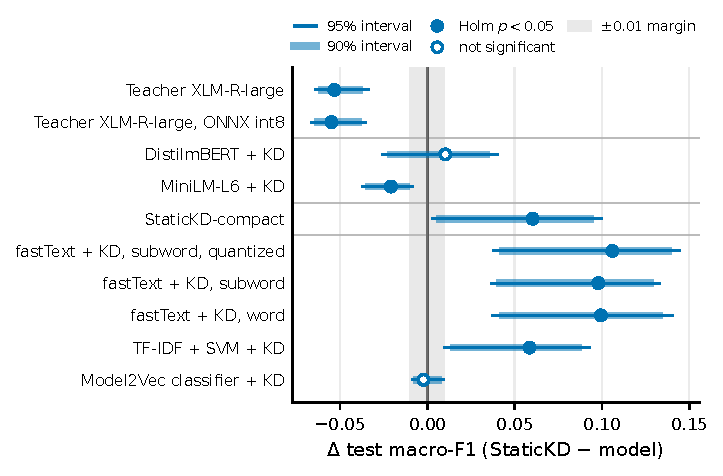
\includegraphics[width=\columnwidth]{figures/fig_sig_forest.pdf}
\caption{Paired difference in test macro-F1 between StaticKD and each other model (StaticKD minus model). Thin lines show 95\% site-cluster bootstrap intervals. Thick bars show 90\% intervals. Filled markers differ significantly after Holm correction. The shaded band is the $\pm$0.01 equivalence margin. The two fastText models trained on GPT-4o labels lie above +0.4 and are not shown.}
\label{fig:sig-forest}
\end{figure}
The paired tests in Table~\ref{tab:sig} and Fig.~\ref{fig:sig-forest} confirm this ranking. The $\Delta$macro-F1 of StaticKD against the teacher is $-$0.053 [$-$0.065, $-$0.033]. MiniLM-L6 keeps a significant lead ($-$0.021 [$-$0.038, $-$0.008], $p=0.005$). StaticKD and DistilmBERT do not differ significantly (+0.010, $p=1.000$). The 90\% interval [$-$0.023, +0.036] is too wide to show equivalence (TOST $p=0.428$). The McNemar test favors StaticKD over DistilmBERT in accuracy ($p<0.001$) but treats articles from the same site as independent. StaticKD is ahead of the quantized fastText + KD by +0.106 [+0.037, +0.145]. Its advantage over TF-IDF + SVM is +0.059 [+0.009, +0.093] ($p=0.040$). The Model2Vec classifier is the only light model that matches StaticKD. The $\Delta$macro-F1 between the two models is $-$0.002 [$-$0.009, +0.010] with a 90\% interval of [$-$0.008, +0.008] inside the $\pm$0.01 equivalence margin (TOST $p=0.025$).

The macro-F1 of StaticKD is higher than that of fastText + KD in 40 of 47 languages (Wilcoxon $p<0.001$). The advantage over TF-IDF + SVM is narrower. StaticKD has the higher macro-F1 in 31 of 47 languages (Wilcoxon $p=0.003$). Per-language accuracy gives a different picture. StaticKD is higher in 24 languages and lower in 22 (Wilcoxon $p=0.127$). Per-language tests find no consistent difference in either metric between StaticKD and DistilmBERT (Wilcoxon $p=0.604$ for macro-F1 and 0.322 for accuracy) or the Model2Vec classifier ($p=0.358$ and 0.534). StaticKD beats the teacher in only 7 of 47 languages.

The model ranking was also checked against the cluster structure of the test set and against the input length of the transformers. The subset with at most five articles per site and language--label pair keeps 8,139 articles. StaticKD obtains 0.587 on it and the teacher 0.627. Only the order of StaticKD and the Model2Vec classifier (0.583) changes on this subset. Leaving out one source at a time places StaticKD between third and fifth of the nine models (Table~S2 in the supplementary material). Only the Model2Vec classifier and DistilmBERT change places with it. Every fastText and TF-IDF model stays at least 0.028 below StaticKD. Retraining with 512-token inputs raises the test macro-F1 of MiniLM-L6 and DistilmBERT to 0.580 and 0.547. MiniLM-L6 stays ahead of StaticKD ($-$0.035 [$-$0.049, $-$0.021], $p<0.001$). DistilmBERT still does not differ significantly from it ($-$0.002 [$-$0.029, +0.022], $p=0.779$).

\subsection{CPU Efficiency (RQ2)}
\label{sec:res-eff}
\begin{table*}[!t]
\caption{CPU Efficiency on Pinned P-Cores (Sample From the Unified Test Set, 1c/4c = 1/4 Cores)}
\label{tab:eff}
\centering
\scriptsize
\resizebox{\textwidth}{!}{%
\begin{tabular}{@{}lcccccl@{}}
\toprule
Model & Latency p50 / p95, 1c (ms) & Throughput 1c (doc/s) & Throughput 4c (doc/s) & Model RAM (MB) & File (MB) & Dependencies \\
\midrule
Teacher XLM-R-large & 2,816 / 2,894 & 0.34 & 0.97 & 2,950 & 2,136 & torch, transformers \\
Teacher XLM-R-large, ONNX int8 & 1,190 / 1,229 & 0.79 & 2.53 & 1,375 & 537 & onnxruntime, transformers \\
DistilmBERT + KD & 193 / 202 & 5.05 & 15.6 & 1,059 & 516 & onnxruntime, transformers \\
MiniLM-L6 + KD & 56.5 / 61.9 & 16.9 & 48.8 & 1,235 & 408 & onnxruntime, transformers \\
\textbf{StaticKD} & 2.01 / 3.31 & 539 & 1,827 & 501 & 34 & numpy, tokenizers \\
StaticKD-compact & 1.78 / 3.17 & 601 & 2,005 & 277 & 23 & numpy, tokenizers \\
fastText + KD, subword, quantized & 1.93 / 3.21 & 545 & 1,393 & 300 & 18 & fasttext, tokenizers \\
fastText + KD, subword & 2.07 / 3.62 & 489 & 1,184 & 1,122 & 839 & fasttext, tokenizers \\
TF-IDF + SVM + KD & 2.96 / 4.49 & 433 & 865 & 828 & 166 & scikit-learn, tokenizers \\
Model2Vec classifier + KD & 1.99 / 3.22 & 568 & 1,822 & 1,091 & 507 & model2vec, scikit-learn \\
\bottomrule
\end{tabular}}
\end{table*}
The teacher is too slow on CPU for a large stream of articles. StaticKD removes this cost almost entirely (Table~\ref{tab:eff}, Fig.~\ref{fig:tradeoff}, and Fig.~S2 in the supplementary material). The PyTorch fp32 teacher needs 2,816~ms per article on one core and reaches a throughput of 0.34 articles per second. The best CPU configuration for the teacher is ONNX int8 (1,190~ms per article and 0.79 articles per second). Classifying one million articles per day would take 14.7 cores (ONNX int8) to 33.7 cores (PyTorch) for this step alone.

StaticKD needs 2.01~ms per article and can process 539 articles per second per core. Its speed is about 682 times that of the ONNX int8 teacher and 1,572 times that of the PyTorch teacher. MiniLM-L6 and DistilmBERT are about 32 and 107 times slower. The StaticKD file is 16 times smaller than that of the ONNX int8 teacher. A load of one million articles per day needs 0.02 cores. StaticKD uses 501~MB of RAM (mostly for the tokenizer structure) and the compact variant 277~MB. Tokenization takes 98\% of the single-thread prediction time and produces 579 tokens per article on average. Averaging the table rows alone runs at 26,843 articles per second.

The single-core speeds of the light models range from 433 articles per second for TF-IDF + SVM to 601 for the compact variant. The quantized fastText + KD is smaller (18~MB) and uses less RAM (300~MB) than StaticKD but reaches a test macro-F1 of only 0.439. The Model2Vec classifier is the only light model that matches the accuracy of StaticKD (Fig.~\ref{fig:tradeoff}). It needs 507~MB on disk and 1,091~MB of RAM. The single-core throughput of every model deviates from the median of the three sessions by at most 7\%.

\begin{figure}[!t]
\centering
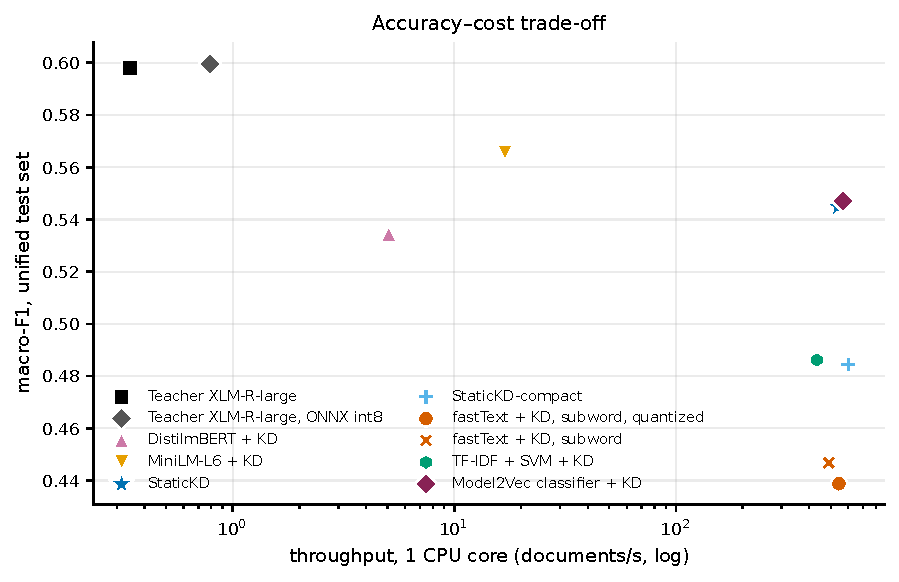
\includegraphics[width=\columnwidth]{figures/fig_tradeoff.pdf}
\caption{Test macro-F1 on the unified test set against single-core CPU throughput (log scale).}
\label{fig:tradeoff}
\end{figure}

\subsection{Ablation, Temperature, and Ensembling (RQ3)}
\label{sec:res-abl}
\begin{table*}[!t]
\caption{Ablations and Temperature (One Student, No Ensemble). Mean $\pm$ Standard Deviation Over Seeds. $^{*}$ = Different From the Final Recipe (Paired Bootstrap, Holm, $p<0.05$). $\Delta$ = Test Macro-F1 Minus That of the Final Recipe [95\% CI]. $^{\dagger}$ = Equivalent Within $\pm$0.01 (TOST)}
\label{tab:ablation}
\centering
\scriptsize
\begin{tabular}{@{}lccccc@{}}
\toprule
Variant & Seeds & Dev macro-F1 & Held-out agreement & Test macro-F1 & $\Delta$ test macro-F1 [95\% CI] \\
\midrule
\multicolumn{6}{@{}l}{\textit{Final recipe}} \\
\quad Final recipe (one seed) & 10 & 0.755$\pm$0.010 & 0.808$\pm$0.001 & 0.542$\pm$0.004 & -- \\
\multicolumn{6}{@{}l}{\textit{Component ablation}} \\
\quad Hard teacher labels (cross-entropy) & 5 & 0.749$\pm$0.007 & 0.805$\pm$0.001 & 0.547$\pm$0.004 & +0.005 [$-$0.002, +0.010]$^{\dagger}$ \\
\quad EMMediaTopic only (4 languages, 20k) & 5 & 0.723$\pm$0.006$^{*}$ & 0.730$\pm$0.001$^{*}$ & 0.491$\pm$0.002$^{*}$ & $-$0.051 [$-$0.064, $-$0.036] \\
\quad 130k documents (no extra CC-News) & 5 & 0.736$\pm$0.009$^{*}$ & 0.799$\pm$0.002$^{*}$ & 0.541$\pm$0.002 & $-$0.002 [$-$0.008, +0.002]$^{\dagger}$ \\
\quad Randomly initialized embedding & 5 & 0.715$\pm$0.005$^{*}$ & 0.739$\pm$0.004$^{*}$ & 0.422$\pm$0.006$^{*}$ & $-$0.120 [$-$0.166, $-$0.047] \\
\quad Frozen embedding (linear head only) & 5 & 0.720$\pm$0.001$^{*}$ & 0.788$\pm$0.001$^{*}$ & 0.557$\pm$0.002 & +0.014 [$-$0.004, +0.024] \\
\quad No token dropout & 5 & 0.757$\pm$0.004 & 0.808$\pm$0.001 & 0.544$\pm$0.002 & +0.001 [$-$0.001, +0.003]$^{\dagger}$ \\
\quad 512-unit MLP head (cannot be folded) & 5 & 0.762$\pm$0.009 & 0.813$\pm$0.002$^{*}$ & 0.551$\pm$0.006 & +0.009 [$-$0.000, +0.012] \\
\multicolumn{6}{@{}l}{\textit{Temperature}} \\
\quad $\tau=0.5$ & 5 & 0.750$\pm$0.004 & 0.807$\pm$0.002 & 0.546$\pm$0.005 & +0.004 [$-$0.002, +0.007]$^{\dagger}$ \\
\quad $\tau=2$ & 5 & 0.748$\pm$0.003 & 0.801$\pm$0.001$^{*}$ & 0.537$\pm$0.001 & $-$0.005 [$-$0.010, +0.008]$^{\dagger}$ \\
\quad $\tau=4$ & 5 & 0.723$\pm$0.004$^{*}$ & 0.791$\pm$0.001$^{*}$ & 0.529$\pm$0.002 & $-$0.014 [$-$0.020, +0.001] \\
\bottomrule
\end{tabular}
\end{table*}
\begin{table}[!t]
\caption{Macro-F1 of Selected Variants by the Amount of Distillation Data in the Language of the Article (Test Set, Mean Over Seeds)}
\label{tab:ablation-groups}
\centering
\footnotesize
\setlength{\tabcolsep}{3pt}
\resizebox{\columnwidth}{!}{%
\begin{tabular}{@{}lcccc@{}}
\toprule
Variant & Dev & Sufficient ($\ge$500) & Few ($<$500) & None (0) \\
\midrule
Final recipe (one seed) & 0.755 & 0.615 & 0.482 & 0.403 \\
Frozen embedding (linear head only) & 0.720 & 0.607 & 0.541 & 0.440 \\
Randomly initialized embedding & 0.715 & 0.567 & 0.182 & 0.161 \\
EMMediaTopic only (4 languages, 20k) & 0.723 & 0.559 & 0.466 & 0.351 \\
Hard teacher labels (cross-entropy) & 0.749 & 0.617 & 0.482 & 0.410 \\
512-unit MLP head (cannot be folded) & 0.762 & 0.613 & 0.484 & 0.421 \\
$\tau=2$ & 0.748 & 0.612 & 0.476 & 0.363 \\
\bottomrule
\end{tabular}}
\end{table}
\begin{figure}[!t]
\centering
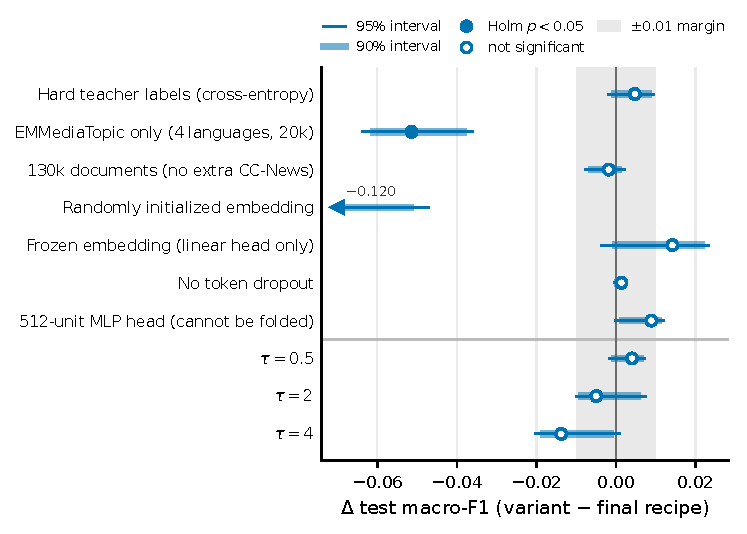
\includegraphics[width=\columnwidth]{figures/fig_ablation_forest.pdf}
\caption{Difference in test macro-F1 between each ablation variant and the final recipe (variant minus final recipe). The encoding follows Fig.~\ref{fig:sig-forest}. A separator divides the component ablations from the temperatures.}
\label{fig:abl-forest}
\end{figure}
Table~\ref{tab:ablation} and Fig.~\ref{fig:abl-forest} report the ablation results with five seeds per variant. Most of the accuracy comes from two components: multilingual distillation data and the pre-trained embeddings. A student distilled on EMMediaTopic alone (4 languages) loses 0.051 in test macro-F1 and 0.077 in held-out agreement. Random initialization in place of potion lowers the test macro-F1 more than any other variant (0.120, $p<0.001$). Only these two variants differ significantly from the final recipe in test macro-F1.

Freezing the embeddings restricts training to the linear head on top of potion and gives mixed results. The development score drops by 0.035 ($p=0.040$) and the held-out agreement by 0.020 ($p<0.001$). The test macro-F1 rises by 0.014 with an interval that includes zero ([$-$0.004, +0.024], $p=1.000$). Table~\ref{tab:ablation-groups} traces the gain to languages with little distillation data (+0.059) and to languages without distillation data (+0.037). The frozen embeddings are slightly weaker in languages with at least 500 documents ($-$0.007).

None of the other variants changes the test macro-F1 significantly. Hard labels from the teacher raise the test macro-F1 by 0.005 ($p=1.000$) and lower the development score by 0.006 ($p=1.000$). The 90\% interval of the test difference lies inside the equivalence margin ([$-$0.001, +0.009], TOST $p=0.017$). Hard labels therefore work as well as soft labels. Reducing the data to 130 thousand documents lowers the test score by 0.002 ($p=1.000$) and the held-out agreement by 0.009 ($p<0.001$). Removing token dropout gives +0.001 ($p=1.000$) and an MLP head that cannot be folded +0.009 ($p=0.780$). The data and dropout variants also pass the equivalence test. The MLP head fails it because its 90\% interval reaches +0.012.

A higher temperature does not help (Fig.~S3 in the supplementary material). The common choice of $\tau=2$~\cite{hinton2015distilling} lowers the held-out agreement by 0.007 ($p<0.001$) compared with $\tau=1$. Neither the test macro-F1 nor the development score changes significantly ($-$0.005 and $-$0.006, both $p=1.000$). The test difference passes the equivalence test at both $\tau=2$ and $\tau=0.5$. The value $\tau=4$ lowers the development score and the held-out agreement significantly. Its test score falls by 0.014 but not significantly ($p=0.836$).

Fig.~S4 in the supplementary material shows the effect of the ensemble size. Three seeds instead of one raise the test macro-F1 from 0.542 to 0.544 and the held-out agreement from 0.808 to 0.810. Ten seeds give 0.546. The gain is small but free at inference time because an ensemble of any size folds into one table.

\subsection{Analysis by Language, Label, and Source (RQ4)}
\label{sec:res-lang}
Table~\ref{tab:groups} and Fig.~S5 in the supplementary material report the share of the teacher score that StaticKD keeps. The share varies more with the amount of distillation data in the language of the article than with the type of label. The share ranges across label origins from 89.5\% for publisher categories to 95.8\% for JSON-LD sections. It falls from 97.5\% in languages with at least 500 distillation documents to 72.3\% in languages without distillation data. The Model2Vec classifier is slightly ahead of StaticKD in the languages without distillation data (0.429 against 0.402). The two classifiers differ by at most 0.011 in every other subgroup of Table~\ref{tab:groups}.

\begin{table*}[!t]
\caption{Test Macro-F1 by Subgroup. Last Column: StaticKD Macro-F1 as a Percentage of the Teacher Macro-F1 in the Same Subgroup}
\label{tab:groups}
\centering
\scriptsize
\setlength{\tabcolsep}{3.5pt}
\begin{tabular}{@{}lrccccccccc@{}}
\toprule
Subgroup & $n$ & Teacher & DistilmBERT & MiniLM & \textbf{StaticKD} & Model2Vec & fastText (q) & TF-IDF+SVM & fastText GPT & \% teacher \\
\midrule
\multicolumn{11}{@{}l}{\textit{Label origin}} \\
\quad human annotation & 4,094 & 0.463 & 0.436 & 0.436 & 0.414 & 0.414 & 0.328 & 0.393 & 0.027 & 90\% \\
\quad publisher category & 2,600 & 0.702 & 0.498 & 0.674 & 0.629 & 0.632 & 0.300 & 0.330 & 0.063 & 90\% \\
\quad JSON-LD section & 6,050 & 0.651 & 0.629 & 0.634 & 0.624 & 0.618 & 0.582 & 0.609 & 0.136 & 96\% \\
\multicolumn{11}{@{}l}{\textit{Distillation data of the language}} \\
\quad sufficient ($\ge$500) & 7,644 & 0.633 & 0.617 & 0.616 & 0.618 & 0.611 & 0.575 & 0.593 & 0.116 & 98\% \\
\quad few ($<$500) & 2,243 & 0.537 & 0.344 & 0.496 & 0.478 & 0.475 & 0.195 & 0.227 & 0.037 & 89\% \\
\quad none (0) & 2,857 & 0.557 & 0.452 & 0.502 & 0.402 & 0.429 & 0.176 & 0.230 & 0.048 & 72\% \\
\multicolumn{11}{@{}l}{\textit{Region}} \\
\quad Africa & 3,044 & 0.697 & 0.532 & 0.576 & 0.542 & 0.550 & 0.325 & 0.408 & 0.085 & 78\% \\
\quad South Asia & 2,681 & 0.575 & 0.410 & 0.544 & 0.509 & 0.510 & 0.241 & 0.276 & 0.046 & 88\% \\
\quad East/Southeast Asia \& Middle East & 1,574 & 0.636 & 0.620 & 0.621 & 0.622 & 0.612 & 0.555 & 0.629 & 0.085 & 98\% \\
\quad Europe & 5,445 & 0.653 & 0.637 & 0.638 & 0.638 & 0.631 & 0.598 & 0.610 & 0.136 & 98\% \\
\multicolumn{11}{@{}l}{\textit{Teacher pre-training coverage}} \\
\quad outside XLM-R pre-training & 1,750 & 0.719 & 0.586 & 0.620 & 0.501 & 0.495 & 0.346 & 0.457 & 0.086 & 70\% \\
\quad in XLM-R pre-training & 10,994 & 0.609 & 0.549 & 0.585 & 0.576 & 0.572 & 0.471 & 0.503 & 0.096 & 95\% \\
\multicolumn{11}{@{}l}{\textit{Site diversity}} \\
\quad diverse ($\ge$10) & 5,225 & 0.657 & 0.642 & 0.643 & 0.642 & 0.637 & 0.601 & 0.616 & 0.134 & 98\% \\
\quad single publisher ($<$3) & 6,204 & 0.517 & 0.387 & 0.475 & 0.433 & 0.435 & 0.224 & 0.287 & 0.045 & 84\% \\
\quad medium (3--10) & 1,315 & 0.559 & 0.556 & 0.539 & 0.543 & 0.532 & 0.503 & 0.533 & 0.089 & 97\% \\
\bottomrule
\end{tabular}
\end{table*}

Table~S3 in the supplementary material splits the test set by source. MN-DS is the only source that is annotated directly with IPTC topics. StaticKD keeps 97.4\% of the teacher score on MN-DS (0.535 against 0.549). The macro-F1 of the teacher itself is lower on this source than on any other source. StaticKD keeps the smallest share on MasakhaNEWS (80.0\%). The human labels of MasakhaNEWS follow a non-IPTC scheme. Eleven of the 16 MasakhaNEWS languages are absent from the distillation data. Bangla is also absent from the distillation data and shows most clearly what the pre-trained embeddings contribute. Both fastText + KD and TF-IDF + SVM collapse on Bangla news (0.191 and 0.010). StaticKD reaches 0.748 on the same articles.

The accuracy of StaticKD is close to that of the teacher in a typical language. The median per-language accuracy gap is $-$0.024 (Fig.~\ref{fig:lang}). Table~S4 in the supplementary material relates this gap to properties of the language. The held-out agreement of StaticKD with the teacher rises with teacher confidence ($\rho=0.71$, $p<0.001$). Its relation to the log amount of distillation data ($\rho=0.31$) is not significant after Holm correction ($p=0.067$). Agreement does not differ significantly across scripts (Kruskal--Wallis $H=10.37$, $p=0.067$). The accuracy gap on the test set narrows as the amount of distillation data grows ($\rho=0.52$, $p<0.001$). The weak spot of StaticKD is a group of African languages. StaticKD reaches a mean accuracy of only 0.407 on languages that lie outside XLM-R pre-training and are also absent from the distillation data (ig, lg, ln, pcm, rn, sn, ti, yo). The teacher reaches 0.643 on the same languages.

Four Indian languages (bn, ml, or [Odia], pa) show how StaticKD behaves on text whose tokens hardly ever appeared in training. At least 67\% of the token occurrences in these languages come from tokens that appear fewer than 10 times in the distillation data. StaticKD still reaches a mean accuracy of 0.624 there compared with 0.738 for the teacher. The compact variant removes these rare tokens from the tokenizer. The accuracy of the compact variant on these four languages falls to 0.013. Accuracy in the other languages is 0.578 for the compact variant and 0.640 for the full StaticKD.

\begin{figure*}[!t]
\centering
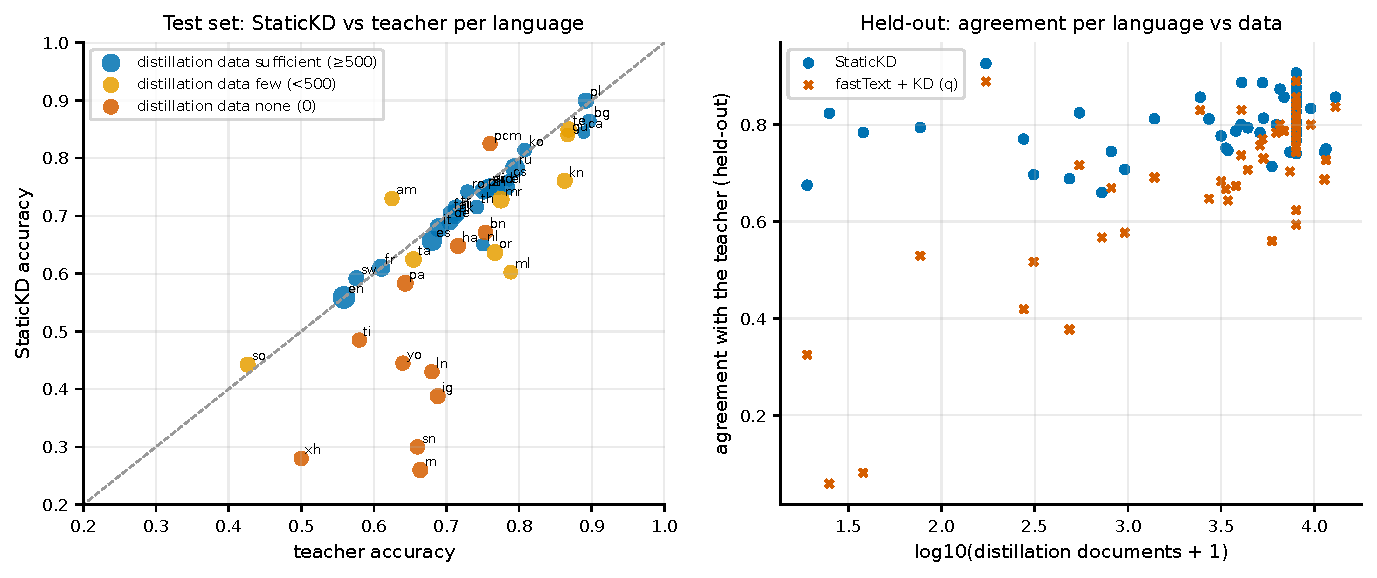
\includegraphics[width=0.8\textwidth]{figures/fig_per_language.pdf}
\caption{Left: StaticKD accuracy against teacher accuracy per test language (color shows the distillation data of the language, size the number of articles). Right: held-out agreement per language against the amount of distillation data for StaticKD and fastText + KD.}
\label{fig:lang}
\end{figure*}

Fig.~S6 in the supplementary material shows the results per label. The hardest labels for StaticKD are \emph{society} (0.16), \emph{disaster} (0.29), \emph{human interest} (0.32), and \emph{conflict} (0.37). The same four labels rank among the hardest for the teacher. StaticKD does best on \emph{sport} (0.88), \emph{weather} (0.84), and \emph{education} (0.75). The largest gaps to the teacher occur for \emph{environment} ($-$0.17), \emph{religion} ($-$0.15), and \emph{arts} ($-$0.08). The most frequent confusions are \emph{society} $\rightarrow$ \emph{human interest}, \emph{human interest} $\rightarrow$ \emph{arts}, and \emph{society} $\rightarrow$ \emph{politics} at 20\% each.

The token table of StaticKD also shows which tokens carry the topic signal of an article. Keeping only the 10\% most specific tokens of each article leaves the test macro-F1 almost unchanged (0.543 with about 58 tokens per article against 0.545 with all tokens). A random 10\% of the tokens gives only 0.435.

\subsection{Calibration and Cascade Mode}
\begin{table}[!t]
\caption{Cascade StaticKD $\rightarrow$ ONNX Int8 Teacher on the Test Set (Effective Single-Core Throughput)}
\label{tab:cascade}
\centering
\footnotesize
\setlength{\tabcolsep}{2.5pt}
\resizebox{\columnwidth}{!}{%
\begin{tabular}{@{}lccccc@{}}
\toprule
$\theta$ & StaticKD share & Accuracy on share & Macro-F1 & Accuracy & doc/s \\
\midrule
0 (StaticKD only) & 100.0\% & 0.641 & 0.545 & 0.641 & 539 \\
0.5 & 80.8\% & 0.732 & 0.586 & 0.690 & 4.09 \\
0.6 & 74.0\% & 0.760 & 0.593 & 0.697 & 3.02 \\
0.7 & 67.4\% & 0.788 & 0.600 & 0.702 & 2.41 \\
0.8 & 60.3\% & 0.813 & 0.602 & 0.703 & 1.98 \\
0.9 & 51.7\% & 0.839 & 0.602 & 0.703 & 1.63 \\
Teacher only & 0.0\% & -- & 0.600 & 0.699 & 0.79 \\
\bottomrule
\end{tabular}}
\end{table}
The ECE of StaticKD is lower than that of the teacher. It is 0.041 on the development set and 0.139 on the test set against 0.090 and 0.245 for the teacher. Both models become overconfident on the out-of-distribution test set (Fig.~S7 in the supplementary material). Table~\ref{tab:cascade} reports the results of the cascade mode. StaticKD decides 60.3\% of the articles at $\theta=0.8$ with an accuracy of 0.813. The cascade reaches an overall accuracy of 0.703 and a macro-F1 of 0.602 against 0.699 and 0.600 for the teacher alone. Its effective throughput is 1.98 articles per second per core and 2.5 times that of the teacher (0.79).

\section{Discussion}
\label{sec:discussion}
\subsection{What a Token Table Retains}
The results in Sections~\ref{sec:res-acc} and~\ref{sec:res-eff} show that a table lookup keeps about nine tenths of the teacher macro-F1. The lookup cuts inference time by about three orders of magnitude. The finding agrees with the observation of~\cite{galke2022bow} that order-free representations are already competitive for topic classification. The token analysis in Section~\ref{sec:res-lang} explains why a table suffices. Almost all of the topic signal in an article is carried by a small share of topic-specific tokens. The remaining gap to the teacher lies in a few labels and in languages that are underrepresented in the distillation data (Table~\ref{tab:groups}). StaticKD falls furthest behind the teacher on \emph{environment}, \emph{religion}, and \emph{arts} (Fig.~S6 in the supplementary material). The lowest StaticKD scores occur on a different set of labels: \emph{society}, \emph{disaster}, \emph{human interest}, and \emph{conflict}. The same labels rank among the hardest for the teacher (Section~\ref{sec:res-lang}). \emph{Society} and \emph{human interest} are known to be difficult even for human annotators~\cite{kuzman2025llm}. The low scores on these labels are therefore not specific to the student.

MiniLM-L6 and DistilmBERT learn from the same distillation data. Only MiniLM-L6 closes part of the gap to the teacher (Table~\ref{tab:sig}). The two models have different origins: MiniLM comes from a distillation of XLM-R-large and DistilmBERT from mBERT. The contrast points to the quality of the initial multilingual representation because both students have six layers. Both models run 32 to 107 times slower than StaticKD on one core.

The Model2Vec classifier reaches the same test macro-F1 as StaticKD within the equivalence margin of $\pm$0.01. The margin is less than half of the gap between StaticKD and MiniLM-L6 (Table~\ref{tab:sig}). It starts from the same potion embeddings and learns from the top teacher label on the same data. It also learns a weight for each token and adds a hidden layer of 512 units. The ablations in Section~\ref{sec:res-abl} show no gain from these extras either. Hard labels are equivalent to soft labels in test macro-F1. The MLP head gives no significant gain in test macro-F1. The accuracy of both models likely comes mainly from the shared embeddings and the teacher-labeled data rather than from the head. The two models run at a similar speed but differ in deployed form. StaticKD folds into one table of 34~MB that needs only \texttt{numpy} and \texttt{tokenizers}. The Model2Vec classifier keeps the full embeddings and its MLP in a 507-MB file and needs about twice the RAM of StaticKD (Table~\ref{tab:eff}).

\subsection{Where the Accuracy Comes From}
The largest contribution comes from the pre-trained multilingual initialization. Random initialization costs 0.120 in test macro-F1 against 0.051 for removing the multilingual data. The multilingual distillation data labeled by the teacher make the second-largest contribution. The most direct evidence for the role of the initialization comes from the compact variant. The four Indian languages bn, ml, or (Odia), and pa hardly occur in the distillation data. Most token occurrences in these languages come from tokens seen fewer than 10 times in the distillation data. The embeddings of these tokens stay close to the potion values because training rarely or never updates such embeddings. The mean accuracy of StaticKD in these languages is still 0.624 but falls to 0.013 once the compact tokenizer removes these tokens. Transfer to languages without data therefore relies on embeddings that training hardly changes. The linear head learned from data-rich languages still applies to such embeddings because the embeddings lie in the same space as the trained ones.

Freezing the embeddings raises the mean scores of languages with little or no distillation data (Table~\ref{tab:ablation-groups}). Fine-tuning moves the embeddings of tokens from the training languages and fits the model better to these languages. Frozen embeddings give a lower development score for this reason. Tokens from other languages stay at the positions assigned by potion. The head of the model has adapted to the moved embeddings and fits the unmoved tokens less well. The final recipe still uses fine-tuning because it was selected on a development set in the training languages. Such a development set cannot reveal this effect. Freezing gives no significant gain on the whole test set but is worth testing for a deployment that targets languages without distillation data.

Soft labels add little or nothing. Hard teacher labels are equivalent to soft labels at $\tau=1$ within $\pm$0.01 macro-F1. A higher temperature never improves on $\tau=1$ (Section~\ref{sec:res-abl}). The pattern fits the literature on the capacity gap~\cite{zhang2025law,wang2026rckd}. A possible explanation is that one linear layer over averaged embeddings cannot represent the inter-class structure in the tail of the teacher distribution (dark knowledge)~\cite{zhao2022dkd}. A high $\tau$ asks the student to imitate a distribution shape beyond its capacity.

\subsection{Weak Languages and Model Selection}
Per-language performance rises with how well a language is represented in the distillation data and the pre-training data. The weakest group consists of African languages outside XLM-R pre-training that are also absent from the distillation data: ig, lg, ln, pcm, rn, sn, ti, and yo. Subwords shared with other languages and sentence context may explain why the teacher still reaches a mean accuracy of 0.643 on these languages. StaticKD reaches only 0.407. The cheapest fix requires no change of architecture. News in these languages can be labeled by the teacher and added to the distillation data. Adding such news is supported by the data ablation and by the correlation between the accuracy gap and the amount of data ($\rho=0.52$).

Agreement with the teacher does not always predict accuracy on editorial labels. Cutting the data to 130 thousand documents lowers the agreement by 0.009 ($p<0.001$) but leaves the test macro-F1 equivalent to that of the final recipe. The frozen-embedding variant scores 0.020 lower in held-out agreement but 0.014 higher in test macro-F1. The test gain is not significant. Student selection should not rely on agreement with the teacher alone~\cite{stanton2021kd}. It should use labels that do not come from the teacher and a development set outside the training distribution.

Test scores should be read with the nature of the labels in mind. An article about a criminal case that involves an athlete can rightly sit in a sports section. A model can label the same article \emph{crime}. Both answers are plausible because IPTC allows several topics per article. The low agreement on MasakhaNEWS comes partly from source categories that are broader than the IPTC target (Section~\ref{sec:res-validity}). Human annotators also disagree often on the \emph{society} label that shows low agreement in MN-DS~\cite{kuzman2025llm}. Comparisons between models remain fair because all models are scored against the same labels.

\subsection{Practical Implications}
Sparse Distillation~\cite{ye2022sparse} uses an n-gram table trained from scratch. StaticKD replaces it with pre-trained multilingual embeddings folded into 17 logits per token. The replacement makes the model smaller and lets it transfer to languages that are missing from the distillation data.

StaticKD suits a real-time pipeline on servers without a GPU. Its output probabilities are better calibrated than those of the teacher. The better calibration makes a cascade mode possible. Such a cascade suits batch jobs that need teacher-level accuracy. The compact variant lowers RAM but is only advisable when all target languages are already covered by the distillation data.

\subsection{Limitations}
\label{sec:limitations}
Section labels from JSON-LD cover 47.5\% of the test articles and publisher categories 20.4\%. Section conventions differ from one publisher to another. A section also reflects one editorial view of an article that may cover several topics at once. The mapping table was built conservatively, validated against the IPTC tree, and reviewed by two researchers in a joint session. A joint review gives no measure of agreement between reviewers. The articles themselves were not re-annotated by humans. Absolute scores on these labels therefore measure agreement with the way publishers categorize articles. The limitation holds especially for \emph{society}, \emph{human interest}, \emph{lifestyle}, and other labels with unclear boundaries.

MasakhaNEWS labels were assigned by human annotators under a non-IPTC scheme and then mapped to IPTC. Direct annotation with IPTC topics exists only in MN-DS and covers English only. The multilingual IPTC test set of Kuzman and Ljube\v{s}i\'c~\cite{kuzman2025llm} is not public.

The number of labels that occur in each language is uneven. The median is 7 labels per language. The African languages cover only three to five broad topics. Per-language scores cannot be compared directly between languages with different label coverage because macro-F1 is computed over the labels present. Publisher diversity is also limited. Twenty-seven languages have fewer than 3 effective sites. Their articles come mostly from MasakhaNEWS, L3Cube-IndicNews, the Bangla news dataset, or one or two CC-NEWS sites. Claims about these languages hold only for those sources. The site-cluster bootstrap widens the confidence intervals of these languages accordingly. All test-set intervals rest on a small number of independent sources because the whole test set has an effective number of only 13.8 clusters.

The teacher bounds the performance of the student from above and passes its errors and biases to the student. The held-out set measures agreement with the teacher and not correctness.

The tuning budget was not equal across models. The StaticKD recipe was fixed on the development set before the test set was built. The fastText and TF-IDF baselines were tuned on the same set with small grids. The Model2Vec classifier used the library defaults. The transformers followed a standard fine-tuning recipe in which only $\tau$ of MiniLM-L6 was searched. Sparse Distillation~\cite{ye2022sparse} was not run as a baseline. It differs from fastText + KD and from the random-initialization ablation in the hidden layers of its deep averaging network, its soft-logit targets, and its billion-parameter n-gram table designed for English. MiniLM-L6 and DistilmBERT read at most 256 tokens in the main comparison. The limit leaves both models less than half of the text of most test articles. Retraining both with 512 tokens raises the test macro-F1 by 0.014 and 0.012 without changing the outcome of the comparison with StaticKD (Section~\ref{sec:res-acc}).

The whole benchmark ran on one machine (Section~\ref{sec:effprotocol}). Latency of the teacher and the transformers was measured on only 100 documents. Absolute numbers will differ on a server but ratios between models measured under the same protocol remain informative.

StaticKD reaches a mean accuracy of only 0.407 on African languages that are absent from both the distillation data and the pre-training data (Section~\ref{sec:res-lang}). A topic filter based on this model could misclassify or drop news in these languages more often. Accuracy should be monitored per language during deployment. Articles with low confidence should be routed to the teacher through the cascade mode.

The scope of this study is limited to top-level IPTC labels and single-label classification. Labels at deeper levels and multi-topic articles have not been tested.

\section{Conclusion}
\label{sec:conclusion}
The open multilingual IPTC classifier needs 1.2 to 2.8 seconds per article on one CPU core. StaticKD distills this classifier into a table of 17 logits per token. The table is initialized from multilingual static embeddings and then trained on 285,999 teacher-labeled articles in 69 languages. The evaluation uses 12,744 test articles in 47 languages whose labels do not come from the teacher. StaticKD reaches a macro-F1 of 0.545 on this set (91.1\% of the teacher score). It processes 539 articles per second per CPU core and is about 682 times faster than the ONNX int8 teacher. The 34-MB model also needs no deep learning library.

The accuracy of this small student comes mainly from multilingual distillation data and pre-trained multilingual embeddings. Soft labels are no better than hard labels. The Model2Vec classifier trained on the same teacher labels is equivalent to StaticKD in test macro-F1 but has a file 15 times larger. Frozen embeddings lower the development score and give higher mean scores in languages with little or no distillation data. The gain on the whole test set is not significant. StaticKD is weakest on languages that appear in neither the distillation data nor the pre-training data of the teacher. Its hardest labels are \emph{society}, \emph{disaster}, \emph{human interest}, and \emph{conflict}. The test set of this study can be reused to evaluate other IPTC classifiers.

The distillation data should be extended to the weak languages and especially to the African languages outside XLM-R pre-training. Fine-tuning could also use a regularizer that keeps the embeddings close to the pre-trained space. Such a regularizer might give in-distribution accuracy and cross-lingual transfer at the same time. Tokenization takes 98\% of the inference time of StaticKD. The next source of speed is therefore a faster tokenizer such as a direct word-to-table lookup. Vocabulary pruning has to keep the rare tokens that languages with little or no distillation data depend on. Several problems remain open: cheap non-linear heads with quantized embeddings, hierarchical classification down to IPTC level 2, multi-label classification, and human IPTC annotation of a multilingual sample of the test set.

\section*{Code, Model, and Data Availability}
The code for this study is available at \todo{GitHub URL and Zenodo DOI}. It covers data collection, test-set construction, teacher labeling, training, evaluation, and benchmarking. The same location provides a notebook that reproduces every number, table, and figure in this paper. The section-to-IPTC mapping table is also released with the code. The StaticKD models are available at \todo{Hugging Face URL}. The test set is released as a manifest of article URLs or IDs, labels, label origins, and text hashes. A reconstruction script comes with the manifest. The article texts themselves are not redistributed because of publisher copyright and the licenses of the source datasets. EMMediaTopic is available from the CLARIN.SI repository~\cite{emmediatopic2025}. Table~S5 in the supplementary material lists the licenses of the assets used and released in this study.

\section*{Acknowledgment}
The authors thank the Department of Informatics Engineering, Sepuluh Nopember Institute of Technology, for supporting this research. The authors used Claude Opus 5.5 (Anthropic) under their direction to explore design options for the method and to run the exploratory and final experiments. It also wrote the experiment code, processed data (including the first draft of the section-to-IPTC mapping table), and drafted parts of the manuscript text. The authors wrote and revised the manuscript themselves, reviewed and verified all code, data, and results, and take full responsibility for its content and claims.

\bibliographystyle{IEEEtran}
\bibliography{references}

\begin{IEEEbiographynophoto}{Obi Kastanya}
\todo{author biography}
\end{IEEEbiographynophoto}

\begin{IEEEbiographynophoto}{Ananta Dwi Prayoga Alwy}
\todo{author biography}
\end{IEEEbiographynophoto}

\EOD

\end{document}
